\subsection{Forza Centripeta}
\textbf{Nota bene: } possiamo ricondurci alla forza centripeta($F_c$) usando le formule per la forza($F = m \cdot a$) e l'accelerazione centripeta($a_c = \frac{v^2}{r} = \omega^2 \cdot r $)! Utilizziamo queste formule per problemi come \textbf{macchine in un circuito di raggio $r$ e coefficiente di attrito dinamico $\mu_d$ dove non deve slittare}.
\\
\begin{gather*}
    \text{Forza centripeta: } F_c = m \frac{v^2}{r} = m \cdot \omega^2 \cdot r
\end{gather*}

\textbf{Nota bene: } se vogliamo che un corpo rimanga nella sua traiettoria circolare, allora la la forza di accelerazione($F_a$)deve essere uguale alla forza centripeta($F_c$).

\begin{center}
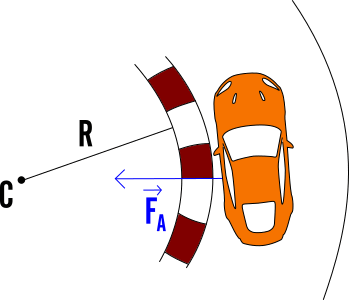
\includegraphics[width=0.7 \linewidth]
{Dinamica/forza-centripeta.png}
\end{center}
\begin{gather*}
    \text{Equivalenza: } F_a = F_c \rightarrow \mu_d  g = \frac{v^2}{r} \\
    \text{Coefficiente d'attrito minimo: } \mu = \frac{v^2}{g \cdot r} \\
    \text{Velocità minima: } v = \sqrt{\mu_d \cdot g \cdot r}
\end{gather*}